\documentclass[12pt, letterpaper]{article}
\usepackage[utf8]{inputenc}

\usepackage{graphicx}
\graphicspath{ {images/} }

\usepackage{amsmath}

\title{First document}
\author{Michael Fedell \thanks{sourced from overleaf.com}}
\date{January 2019}

\begin{document}
\maketitle
We now have a title prepared with author and date.
This \LaTeX{} document is starting to look great!

\newpage

Some of the \textbf{greatest}
discoveries in \underline{science}
were made by \textbf{\textit{accident}}.


In case you didn't catch that,

Some of the greatest \emph{discoveries}
in science
were made by accident.

\textit{Some of the greatest \emph{discoveries}
in science
were made by accident.}

\textbf{Some of the greatest \emph{discoveries}
in science
were made by accident.}

\newpage

The universe is immeense and it seems to be homogeneous, in a large scale, everywhere we look.

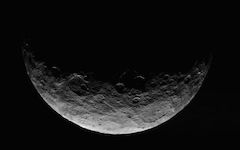
\includegraphics{moon}

There's a picture of the moon above

\newpage

\begin{figure}[h]
    \centering
    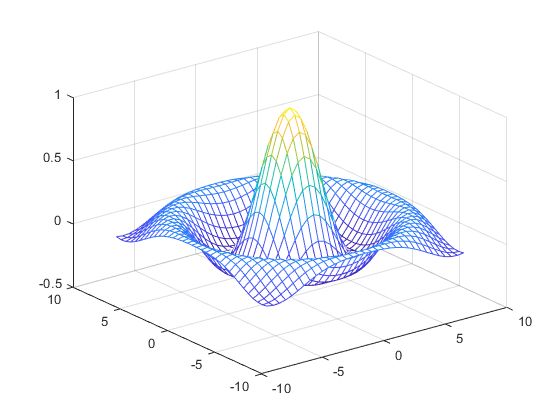
\includegraphics[width=0.25\textwidth]{mesh}
    \caption{a nice plot}
    \label{fig:mesh1}
\end{figure}

As you can see in the figure~\ref{fig:mesh1}, the
function grows near 0. Also, in the page~\pageref{fig:mesh1}
is the same example.

\newpage

\begin{itemize}
    \item The individual entries are indicated with a black dot, a so-called bullet.
    \item The text in the entries may be of any length.
\end{itemize}

\begin{enumerate}
    \item This is the first entry in our list
    \item The list numbers increase with each entry we add
\end{enumerate}

\newpage

In physics, the mass-energy equivalence is stated
by the equation $E=mc^2$, discovered in 1905 by Albert Einstein.

The mass-energy equivalence is described by the famous equation

\[E=mc^2\]

discovered in 1905 by Albert Einstein.
In natural units ($c = 1$), the formula expresses the identity

\begin{equation}
E=m
\end{equation}

Subscripts in math mode are written as $a_b$ and superscripts are written as $a^b$. These can be combined an nested to write expressions such as

$$T^{i_1 i_2 \dots i_p}_{j_1 j_2 \dots j_q} = T(x^{i_1},\dots,x^{i_p},e_{j_1},\dots,e_{j_q})$$

We write integrals using $\int$ and fractions using $\frac{a}{b}$. Limits are placed on integrals using superscripts and subscripts:

$$\int_0^1 \frac{1}{e^x} =  \frac{e-1}{e}$$

Lower case Greek letters are written as $\omega$ $\delta$ etc. while upper case Greek letters are written as $\Omega$ $\Delta$.

Mathematical operators are prefixed with a backslash as $\sin(\beta)$, $\cos(\alpha)$, $\log(x)$ etc.

\newpage

\end{document}